\documentclass[letter]{article}

\usepackage[margin=1in]{geometry} % make more efficient use of the page

\usepackage[utf8]{inputenc}

\usepackage{amsmath} % math tools
\usepackage{amsfonts} % math tools
\RequirePackage{amssymb} % math tools
\RequirePackage{amsbsy} % math tools

\renewcommand{\vec}[1]{\ensuremath{\boldsymbol{#1}}} % make vectors nicer

\usepackage{graphicx} % graphics
\usepackage{xcolor} % colored text

\usepackage{hyperref} % URLs and such
\usepackage{verbatim} % allows \verb-- command

\usepackage{algorithmicx} % algorithm environment
\usepackage{listings} % code listings

\usepackage{natbib} % bibliography

\newcommand{\mypath}[1]{\texttt{\path{#1}}}
\newcommand{\cmd}[1]{\begin{quote}\texttt{> #1}\end{quote}}


\title{CMDA 3634 \\ Lab 05 Report}
\author{Russell J. Hewett}
\date{}


\begin{document}

\maketitle

    \begin{enumerate}
        \item Answer the following questions about your laptop computer.  You will need to refer to Internet resources for this information.  You must cite your sources.  Note, the mechanisms to find the answers to these questions are different for Windows vs macOS.  Find this information for your laptop, not for the VM.
            \begin{itemize}
                \item What brand, model, and version is your processor?
                \item What size are the L1, L2, L3 (if it exists) caches?
                \item How many bytes per cache line? 
                \item How big is your main memory?
            \end{itemize}
        
        \textbf{ANSWER:} % answer goes here
        Some data from \url{https://en.wikichip.org/wiki/intel/core_i7/i7-7700hq} and \url{http://www.cpu-world.com/CPUs/Core_i7/Intel-Core%20i7%20i7-7700HQ.html}.
        \begin{tabular}{lll}
                    & Host OS     & Guest OS \\
        Brand       & Intel       & Intel    \\
        Model       & Core i7     & Core i7  \\
        Version     & 7700HQ      & 7700HQ   \\
        L1          & 32KB (data) & 32KB (data) \\
        L2          & 256KB/core  & 256KB \\
        L3          & 6MB         & 611KB \\
        Cache-line  & 64B         & N/A \\
        Main Memory & 16GB        & 4GB
        \end{tabular}

        \item In the command line on your virtual machine, you can check information about the processor by checking the contents of the /proc/cpuinfo file: \cmd{cat /proc/cpuinfo}
        Copy this information into a table. Does this match your laptop's 
        processor? 
        
        \textbf{ANSWER:} % answer goes here

        See above.  Everything matches except for the main memory, which we configured to be smaller in the VM.
        
        \item In your own words, describe the difference between the two calculations being timed in \texttt{matvecColOrient.c} and \texttt{matvecRowOrient.c}. Before running any code, can you make any predictions about their relative performance for different sized matrices? 
        
        \textbf{ANSWER:} % answer goes here

        The row-oriented calculation loops over rows first, then columns and the column-oriented calculation loops over columns first, then the rows.  The row-oriented version should be faster because the matrix array is indexed in row-major order.
        
        \item We will analyze square matrices for this exercise, although the code allows for rectangular matrix studies. Say that you were to perform a matrix-vector multiplication $\vec{A}\vec{x} = \vec{b}$, where $\vec{A} \in \mathbb{R}^{N\times N}$, and $\vec{x}, \vec{b} \in \mathbb{R}^N$. 
            \begin{enumerate}
                \item Write a general formula for how many bytes of data you expect this to use (similar to the $16N$ expression used in the random-order axpy example in class).
                \item For your system, at what value for $N$ do you expect to exceed L1 cache? 
                \item For your system, at what value for $N$ do you expect to move out of lower level (L2 or L2+L3) cache? 
            \end{enumerate}
        
        \textbf{ANSWER:} % answer goes here

            \begin{enumerate}
                \item The \vec{A} has $N^2$ 4-byte floats and \vec{x} ans \vec{b} have $N$ 4-byte floats.  Thus, the total data used would be $4(2N+N^2)$ Bytes, ignoring loop indicies.
                \item $4(2N+N^2) B= 32*1024B \implies N \approx 89$.
                \item $4(2N+N^2) B= (256+32)*1024B + 6144*1024B \implies N \approx 1279$.
            \end{enumerate}

        
        \item Using the experiment script \mypath{cache_row_orient.sh}, record the results for \texttt{matvecRowOrient.c} in the table below, to analyze the cache performance for this data access pattern. 
        
        \textbf{ANSWER:} % answer goes here

        \begin{center}
        \begin{tabular}{|l | c |  c | c | c | c | c |} 
        \hline
        \textbf{nRows} & \textbf{nCols} & \textbf{ time (s)} &  L1 read miss $\%$ & LL read miss $\%$  &  L1 write miss $\%$ & LL write miss $\%$ \\ \hline
        10    & 10    & 0.0000003800 & 1.6\% & 1.3\% & 2.9\% & 2.6\% \\
        20    & 20    & 0.0000013000 & 0.5\% & 0.4\% & 1.7\% & 1.4\% \\
        40    & 40    & 0.0000052200 & 0.2\% & 0.1\% & 0.6\% & 0.6\% \\
        80    & 80    & 0.0000255400 & 0.0\% & 0.0\% & 0.3\% & 0.2\% \\
        160   & 160   & 0.0000896800 & 0.3\% & 0.0\% & 0.3\% & 0.1\% \\
        320   & 320   & 0.0003911600 & 0.3\% & 0.0\% & 0.2\% & 0.1\% \\
        640   & 640   & 0.0015848800 & 0.3\% & 0.0\% & 0.2\% & 0.1\% \\
        1280  & 1280  & 0.0066128600 & 0.3\% & 0.2\% & 0.2\% & 0.1\% \\ 
        2560  & 2560  & 0.0249078800 & 0.3\% & 0.3\% & 0.2\% & 0.2\% \\
        5120  & 5120  & 0.1010645400 & 0.6\% & 0.3\% & 0.2\% & 0.2\% \\\hline
        \end{tabular}
        \end{center}
        

        \item Using the experiment scripts \mypath{cache_col_orient.sh}, record the results for \texttt{matvecColOrient.c} in the table below, to analyze the cache performance for this data access pattern. 
        
        \textbf{ANSWER:} % answer goes here

        \begin{center}
        \begin{tabular}{|l | c | c | c  | c | c | c |} 
        \hline
        \textbf{nRows} & \textbf{nCols} & \textbf{time (s)} & L1 read miss $\%$ & LL read miss $\%$ &  L1 write miss $\%$ & LL write miss $\%$\\ \hline
        10    & 10    & 0.0000003800 & 1.6\% & 1.3\% & 2.9\% & 2.6\% \\
        20    & 20    & 0.0000014800 & 0.5\% & 0.4\% & 1.7\% & 1.4\% \\
        40    & 40    & 0.0000054200 & 0.2\% & 0.1\% & 0.6\% & 0.6\% \\
        80    & 80    & 0.0000249200 & 0.0\% & 0.0\% & 0.3\% & 0.2\% \\
        160   & 160   & 0.0000892000 & 0.3\% & 0.0\% & 0.2\% & 0.1\% \\
        320   & 320   & 0.0004509200 & 4.9\% & 0.0\% & 0.2\% & 0.1\% \\
        640   & 640   & 0.0029247200 & 4.9\% & 0.0\% & 0.2\% & 0.1\% \\
        1280  & 1280  & 0.0154923400 & 4.9\% & 0.2\% & 0.2\% & 0.1\% \\ 
        2560  & 2560  & 0.1498281800 & 4.9\% & 0.3\% & 0.2\% & 0.2\% \\
        5120  & 5120  & 0.8327762400 & 4.9\% & 4.9\% & 0.2\% & 0.2\% \\\hline
        \end{tabular}
        \end{center}
        
        
        \item Using your favorite plotting software (Excel, Python Matplotlib, Plot.ly, Matlab, etc.) plot the timing results for each of the above tables.  You should plot $N$ on the x-axis and the run-time on the y-axis.  Both axes should use a logarithmic scale.

        Be sure to add any files/code used to produce the plot in your \mypath{lab05/report} folder.  Your plot must have a legend indicating which series corresponds to which experiment.  
        
        \textbf{ANSWER:} % answer goes here
        
        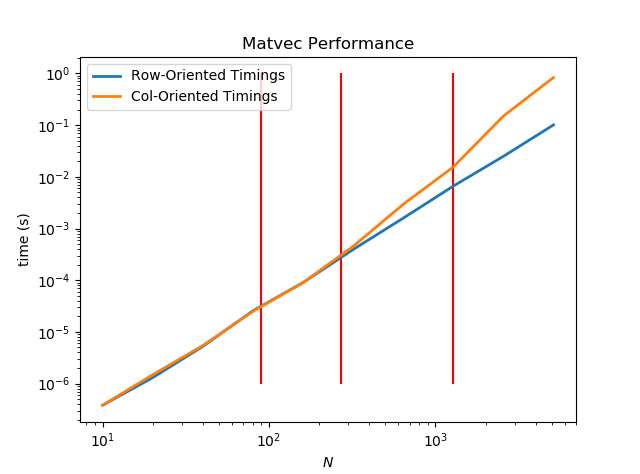
\includegraphics{timing.png}

        Code is in \texttt{plot\_data.py}

        \item In the previous plot, where are the noticeable changes in the timing trends?   At the point(s) where the timing trends change, what is causing this change?  Support your argument with your memory size predictions and your cachegrind data. You may need to take more samples.  Be sure to include any additional code/files used to produce those figures in your \texttt{lab05/report} folder.
        
        \textbf{ANSWER:} % answer goes here
        
        The red lines in the plot indicate the values of the cache boundaries (L1, L2, L3) from problem 4.  In these areas we notice a change in the timing trends for the column-oriented algorithm.  For the row-oriented algorithm we do not see these trends as the access patterns map well to the cache and prefetching behavior.

        \item How many processors does your virtual machine have? How do you know? Include a screenshot if it's useful. 
        
        \textbf{ANSWER:} % answer goes here

        The VM is configured to 1 processor.  This info came from \texttt{lscpu}.
       
        \item In the table below, record your timing results for the serial matrix-vector multiply (with row-major access) and for the openmp matrix-vector multiply (with row-major access).   Also, record the ratio of the times.

        Did you get as much speedup as you expected based on the number of processors? Why do you think this happened?
        
        \textbf{ANSWER:} % answer goes here

         \begin{center}
        \begin{tabular}{|l | c | c | c |c |} 
        \hline
        \textbf{nRows} & \textbf{nCols} & \textbf{time (s) without omp} & \textbf{time (s) with omp} & \textbf{serial time / omp time} \\ \hline
        10   & 10   & 0.0000003773 & 0.0000009947 & 0.38 \\
        20   & 20   & 0.0000020441 & 0.0000046239 & 0.44 \\
        40   & 40   & 0.0000057851 & 0.0000060627 & 0.95 \\
        80   & 80   & 0.0000363203 & 0.0000222913 & 1.63 \\
        160  & 160  & 0.0002472032 & 0.0001031512 & 2.40 \\
        320  & 320  & 0.0008854729 & 0.0004679907 & 1.89 \\
        640  & 640  & 0.0035193957 & 0.0016044020 & 2.19 \\
        1280 & 1280 & 0.0097061886 & 0.0065218148 & 1.49 \\
        2560 & 2560 & 0.0276844027 & 0.0270949682 & 1.02 \\
        5120 & 5120 & 0.1148509079 & 0.1049633594 & 1.09 \\\hline
        \end{tabular}
        \end{center}

        Initially we did not achieve a speedup of 2, as expected, because the startup cost of the second OpenMP thread were higher than the cost of the single thread doing work (and the problem fit into cache).  Until we exceeded the rough boundary of the cache, we obtained nearly the 2x speedup that was anticipated.  After the problem went to main memory, the performance reduced again, beacuse we crossed into the main memory boundary.

        \item Other than the instructor or TAs, who did you receive assistance from on this assignment?
        
        \textbf{ANSWER:} % answer goes here
        
        No one.

    \end{enumerate}

\end{document}
